\chapter{状態、アイデンティティ、変化}

あなたは、エンティティ、データのコレクション、ドメイン関数、およびシーケンシャルなデータを処理するためのいくつかの便利なパターンを手に入れました。そろそろ、アプリケーションの実行中におけるドメインデータの連続性について考え始める時期です。

つまり、ドメインエンティティのIDと状態、そしてドメイン内のIDがどのように関連しているかを考える必要があるのです。ドメイン内で一貫した状態管理を行うことで、第5章「コアの使用」で検討する並行処理のためのアプリケーションを準備することができます。

この章では、ドメイン内のエンティティの状態の変更を管理するためのClojureのツールの適用を学びます。より基本的には、アイデンティティと状態を別々のものとして見ていきます。Clojureは、コンピューティング世界のマルチコア状態を利用するように設計されています。状態管理の戦略を選択するための実用的なアドバイスを見つけ、マルチスレッドプログラムを考慮して、ミュータビリティがもたらす落とし穴のいくつかを認識することを学びます。

Clojureアプリケーションのコンテキストで状態とIDが何を意味するのか、その概要から始めましょう。


\section{変更のモデル化}

Clojureの焦点はimmutableな値であることを思い出してください。不変のデータでは、"更新 "は、その場のエンティティまたはエンティティを更新するのではなく、エンティティ(またはエンティティのコレクション)の新しいインスタンスを生成します。ほとんどの場合、この方法で十分に目的を果たすことができます。時には、アプリケーションの世界の変化をモデル化し、データの変化を追跡する必要があります。具体的には、変更されたデータのセットへの参照を保持する必要があります。

マルチスレッドのシナリオでは、その場でデータを更新することは、多くの複雑な問題を引き起こします。誰がデータを変更できるのか?他のスレッドにはどのように変更が通知されるのか?複数の更新が同時に発生した場合、どのプロセスが優先されるのか?Clojureは、状態管理ツールによって、これらの質問すべてにエレガントな答えを提供します。これらのツールを効果的に使用するには、まずClojureのアイデンティティと状態へのアプローチを理解する必要があります。

\subsection{スナップショットで見る}

その理解を助けるために、少し時間の話をしましょう。人間の経験は連続的に見えますが、あなたの感覚は情報を個別の量子に分けて収集しています。音、景色、匂いは、それぞれ独立して脳に入り、時間的な瞬間に相関します。その瞬間が連続して再生されることで、連続した知覚が得られると錯覚しているのです。

もし、自分の視覚的な量子を見るなら、次の図に示すエドワード・マイブリッジの「疾走するサリー・ガードナー」のようなスナップショットの連続が見えるだろう。

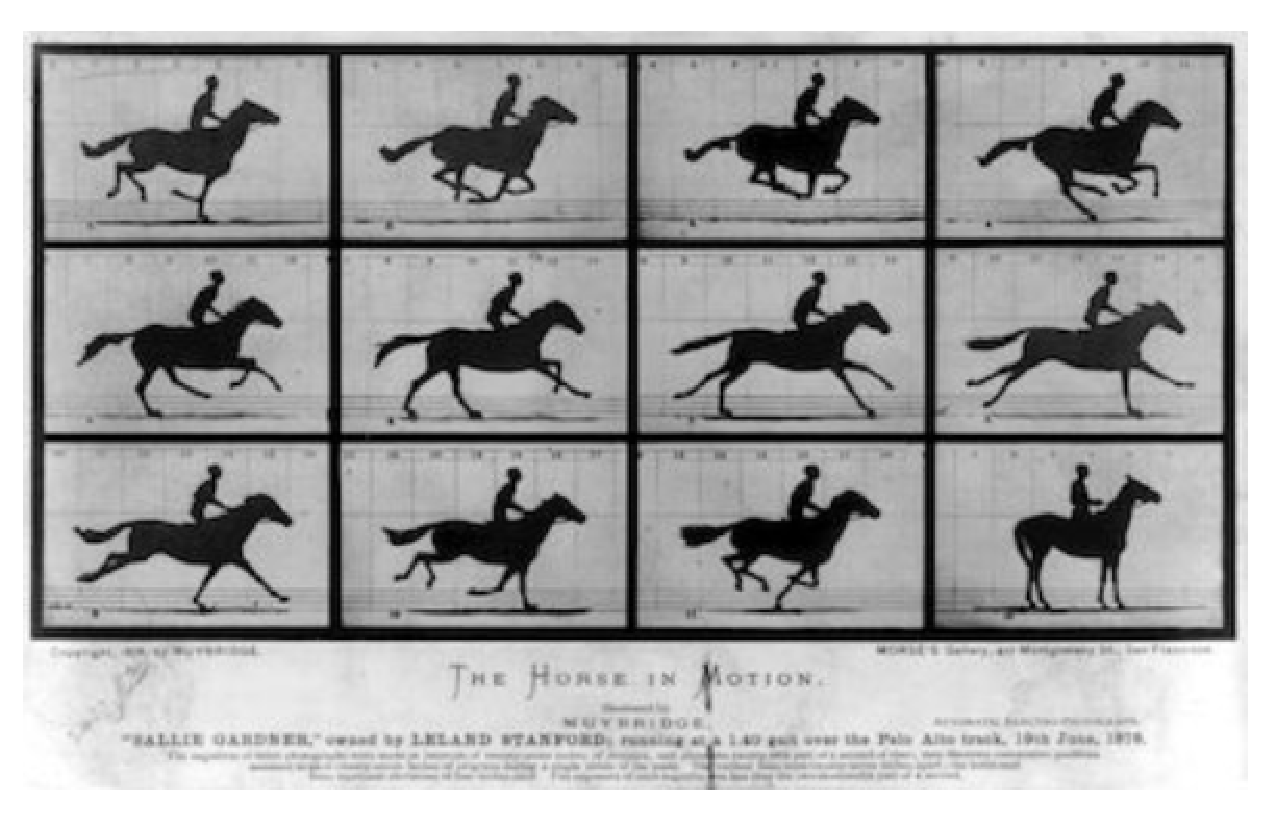
\includegraphics[width=10cm]{fig_04_001.eps}



 % Modeling a Change
\section{変更を管理するためのツール}

Clojureには、アプリケーションの状態を保存するために使用できる4つの参照型(\texttt{var}、\texttt{atom}、\texttt{agent}、\texttt{ref})があります。どの場合にも、メカニズムは、不変の値を格納するミュータブルコンテナを提供します。コンテナは初期値で作成し、その値をリセットすることができます。また、統一更新モデルを用いて状態を進めることもできる。このようにして、アプリケーションの状態を管理された方法で変更することができる。

Clojureの参照型は\texttt{IRef}を実装しています。次の表は、これらの型と、それらの作成、更新、およびリセット関数の一覧です。

\begin{tabular}{|l|l|l|l|}
\hline
IRef & create-fn & update-fn(s) & set-fn \\ \hline \hline
Atom & atom & swap! & reset! \\ \hline
Ref & ref & alter, commute & ref-set \\ \hline
Var & def & alter-var-root & var-set \\ \hline
Agent & agent & send, send-off & restart-agent \\ \hline
\end{tabular}





 % Tools for Managing Change
\section{変化と生きる}

Clojureが提供する、アプリケーションの状態を更新するためのツールをいくつか詳しく見てきました。これらのツールは、変更が有効であり、瞬時に見えることを保証することで、不運から守ってくれます。しかし、まだずさんな考えで自分自身の足を撃つことができます。

状態管理の複雑さを、ドキュメントやブログ記事、そしてこの本のようなおもちゃのようなコードで示すことは困難です。しかし、これまで見てきたような仕組みを応用する際には、いくつかのガイドラインを心に留めておくとよいでしょう。

\subsection{バリデーションの方法とタイミング}

私たちの\texttt{shopping.store} APIは、冗長性と少し厄介な部分を含んでいます。\texttt{init}では、私たちのAPI(特に\texttt{grab})を無視してストアの\texttt{inventory}を直接更新するコードから保護するために、バリデータ関数として在庫に\texttt{no-negative-values?}関数を適用しました。

このバリデータメソッドは、マップのすべての要素を検査して、在庫が増加していることを確認します。在庫が大きくなり始めたらどうなるのでしょうか?\texttt{grab}で使っている\texttt{in-stock?}テストと比較して、どれだけのオーバーヘッドになるでしょうか?厄介なことに加えて、冗長です。\texttt{grab}を使おうが使うまいが、バリデータは呼び出されるのです。

どうすればいいでしょうか?少なくとも、\texttt{inventory}の\texttt{def}に \texttt{^\{:private true\}} を追加して、\texttt{grab} の使用を奨励すべきです。より堅牢な解決策は、システムを初期化する関数を構築し、それを必要とするコンポーネントに渡すことです。これは、第7章「アプリケーションを構成する」で詳しく説明するコンポジションの水域に足を踏み入れることになります。

APIを開発する際には、必要と思われるすべてのアクションをラップした一連の関数を提供し、実際のデータの保存は非公開にするようにしましょう。こうすることで、提供された関数をバイパスして直接データを操作することを防ぐことができます。これにより、バリデータのパフォーマンスが低下するような場面でも、 不正な操作から保護する仕組みを導入することができます。バリデータ関数は Clojure がトランザクションをコミットする前に実行されるので、 長時間実行するバリデータはステートフルなリソースへのリクエストをブロックしたり キューに入れたりする可能性があることを覚えておいてください。

一方、バリデータ関数の定義は、小さなデータやプログラムの状態には効果的です。(たとえば) ロギング用のファイル名を含むアトム設定がある場合、 そのファイルが存在するかどうかをバリデータに確認させたいことがあります。ひとつのアトムでさまざまな更新が可能な場合、バリデータを使用すると検証を一元化でき、 必要なコードの量を減らすことができます。もちろん、誰かがルールを破ったときに発生する例外をキャッチする準備はしておかなければなりませんが、 設計とは常にトレードオフの関係にあるものなのです。

\subsection{ランタイムステートとプログラムステート}

安心してください、これは少しは分ける価値があります。この章では、主にプログラムの状態やアプリケーションの状態について話してきました。つまり、インベントリやショッピングリストなど、問題領域にある管理された状態を対象にしてきました。プログラム状態は、ソフトウェアがモデル化するドメイン知識と、ソフトウェアが解決しようとする問題に直接関連するデータと概念に、管理されたアクセスを提供する役割を果たします。

店舗APIにはinventoryアトムがあり、そこにsold-itemsアトムを後から追加した。家族での買い物は、買い物リスト、割り当て、ショッピングカートを管理した。これらの要素はすべてプログラム・ステートである。プログラムの状態には、可能な限りAPIを使ってアクセスし、直接ではなく、慎重に吟味されたメソッドを通して使用されるべきである。

一方、ランタイムステートは、ソフトウェアの実行を容易にするために存在する。ランタイム状態は、データベース、設定ファイル、ネットワーク接続、または呼び出す予定のコンポーネントへの参照を保持する役割を果たします。これらは動作環境に影響を与えるもので、ドメイン情報には関係ない。ランタイムステートについては、第7章「アプリケーションを構成する」で詳しく説明します。ランタイムステートはしばしば避けられないもので、設定可能性を損なわずに最小化することは困難です。もしソフトウェアが必要とする状態情報の量を削減したいのであれば、代わりにプログラムの状態に注目しましょう。

関数型プログラミングに慣れないうちは、反射的にドメインに不必要なミュータビリティを散りばめてしまいがちです。この傾向は2つの方向から攻めることができます。1つ目は、前もってそれを確認すること、2つ目は、最後に変異性を減らすことです。



 % Living with Change
\section{まとめ}

アプリケーションを構築するとき、私たちはしばしば、そうでなければ純粋なアプリケーションを通して更新を進めていくことに気づきます。もし私たちがルールを明確にし、関数に責任を持ち、管理する必要があるものを正しく選択するならば、効果的にそれを行うことができます。

データとその状態の変化を一連のスナップショットとして見ることで、他のプロセスのオブザーバの存在を考慮した上で、責任ある行動をとることができる。Clojureでは、それらのスナップショットは、ミュータブルな参照に包まれた以前のバージョンとして保持されます。これは、すべてのオブザーバーが特定の瞬間の値の一貫したセットを持っていることを保証し、誰も不幸な状況に自分自身を見つけることはありません。

この章では、時間の観点から見たアイデンティティと状態についてのアイデアを探求することから始めました。これらのアイデアを使用して、Clojure の vars によるグローバルな状態、および atoms と refs を使用して更新を管理する機能について学びました。これらのことはすべて、時間の経過とともにストーリーを整理しておくのに役立ちます。これで、並行処理に進むためのツールを手に入れました。

次の章では、並行処理について考えていきます。また、子供と一緒に買い物に行ったときに見た core.async をより深く見ていきます。エージェントは、私たちの管理対象名簿を完成させるでしょう。 % Wrapping Up